\begin{picture}(0,0)%
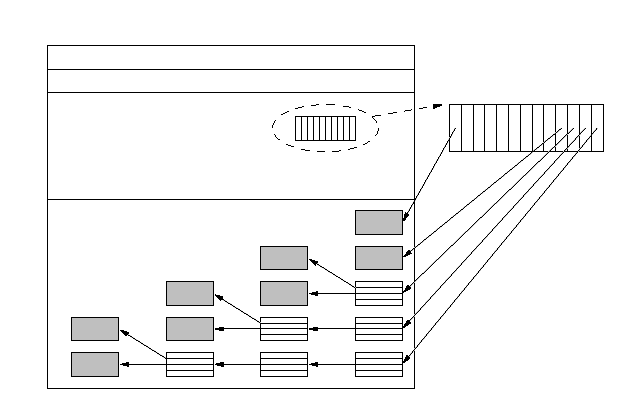
\includegraphics{img/tex/s5}%
\end{picture}%
\setlength{\unitlength}{4144sp}%
%
\begingroup\makeatletter\ifx\SetFigFont\undefined%
\gdef\SetFigFont#1#2#3#4#5{%
  \reset@font\fontsize{#1}{#2pt}%
  \fontfamily{#3}\fontseries{#4}\fontshape{#5}%
  \selectfont}%
\fi\endgroup%
\begin{picture}(4467,2832)(46,-2053)
\put(3331,164){\makebox(0,0)[lb]{\smash{\SetFigFont{10}{12.0}{\sfdefault}{\mddefault}{\updefault}{\color[rgb]{0,0,0}0}%
}}}
\put(4141,164){\makebox(0,0)[lb]{\smash{\SetFigFont{10}{12.0}{\sfdefault}{\mddefault}{\updefault}{\color[rgb]{0,0,0}9}%
}}}
\put(4366,164){\makebox(0,0)[lb]{\smash{\SetFigFont{10}{12.0}{\sfdefault}{\mddefault}{\updefault}{\color[rgb]{0,0,0}12}%
}}}
\put(1336,254){\makebox(0,0)[lb]{\smash{\SetFigFont{10}{12.0}{\sfdefault}{\mddefault}{\updefault}{\color[rgb]{0,0,0}superblock}%
}}}
\put(361, 29){\makebox(0,0)[lb]{\smash{\SetFigFont{10}{12.0}{\sfdefault}{\mddefault}{\updefault}{\color[rgb]{0,0,0}i-node area}%
}}}
\put(361,-781){\makebox(0,0)[lb]{\smash{\SetFigFont{10}{12.0}{\sfdefault}{\mddefault}{\updefault}{\color[rgb]{0,0,0}data block area}%
}}}
\put( 46,659){\makebox(0,0)[lb]{\smash{\SetFigFont{10}{12.0}{\sfdefault}{\mddefault}{\updefault}{\color[rgb]{0,0,0}block number}%
}}}
\put( 91,434){\makebox(0,0)[lb]{\smash{\SetFigFont{10}{12.0}{\sfdefault}{\mddefault}{\updefault}{\color[rgb]{0,0,0}0}%
}}}
\put( 91,254){\makebox(0,0)[lb]{\smash{\SetFigFont{10}{12.0}{\sfdefault}{\mddefault}{\updefault}{\color[rgb]{0,0,0}1}%
}}}
\put( 91, 74){\makebox(0,0)[lb]{\smash{\SetFigFont{10}{12.0}{\sfdefault}{\mddefault}{\updefault}{\color[rgb]{0,0,0}2}%
}}}
\put(113,-91){\rotatebox{270.0}{\makebox(0,0)[lb]{\smash{\SetFigFont{14}{16.8}{\sfdefault}{\mddefault}{\updefault}{\color[rgb]{0,0,0}...}%
}}}}
\put(758,434){\makebox(0,0)[lb]{\smash{\SetFigFont{10}{12.0}{\sfdefault}{\mddefault}{\updefault}{\color[rgb]{0,0,0}boot block}%
}}}
\end{picture}
